\documentclass[../report.tex]{subfiles}
\begin{document}

\graphicspath{{img/}{../img/}}

\section{Activity Breakdown}

\label{sec:Activity Breakdown}

Et Activity Breakdown Diagram laves ved at identificere de aktiviteter, der skal udf�res for at et projekt bliver f�rdigt. Man inddeler alts� projektet i aktiviteter, og n�r alle aktiviteter er udf�rt, er hele projektet udf�rt. Hver aktivitet kan ogs� inddeles i mindre aktiviteter. Ligesom et Product Breakdown Diagram danner disse aktiviteter et hierarki, hvor den �verste aktivitet vil v�re at udf�re hele projektet, og de nederste aktiviteter vil v�re detaljerede aktiviteter, som er mere overskuelige at arbejde med.

Dette g�r det blandt andet nemmere at estimere et projekt, fordi det er lettere at estimere, hvor lang tid det tager at lave en lille del (f.eks. en database), end det er at estimere hvor lang tid et helt projekt tager \cite[p.~133-134]{hughescotterell09}. Det giver ogs� mulighed for at se p� hvordan aktiviteterne afh�nger af hinanden, s� man kan prioritere, hvad der skal laves f�rst. 

I target-projektet blev der lavet et Activity Breakdown Diagram, som ikke br�d aktiviteterne i projektet helt ned i atomiske aktiviteter (se figur \ref{fig:Activity Breakdown Diagram}). Aktiviteterne blev holdt p� et nogenlunde abstrakt niveau, fordi der blev arbejdet med Scrum som procesmodel i target-projektet (se sektion \ref{sec:Scrum}). Det var derfor ikke n�dvendigt at bryde alle aktiviteter ned i atomiske dele i starten af projektet. Den nedbrydning fandt sted l�bende, n�r der blev holdt m�der i forbindelse med sprintplanl�gning. De atomiske aktiviteter, der kom ud af denne nedbrydning, blev brugt som tasks i Scrum. Et eksempel p� en s�dan nedbrydning kan ses p� figur \ref{fig:Full Breakdown Diagram}. Hvis man derimod havde brugt vandfaldsmodellen som procesmodel (se sektion \ref{sec:Vandfaldsmodellen}), havde det v�ret n�dvendigt at nedbryde alle aktiviteter s� meget s� muligt fra starten af projektet, for at kunne estimere bedst muligt.

\begin{figure}[H]
\hspace*{-2.5cm}
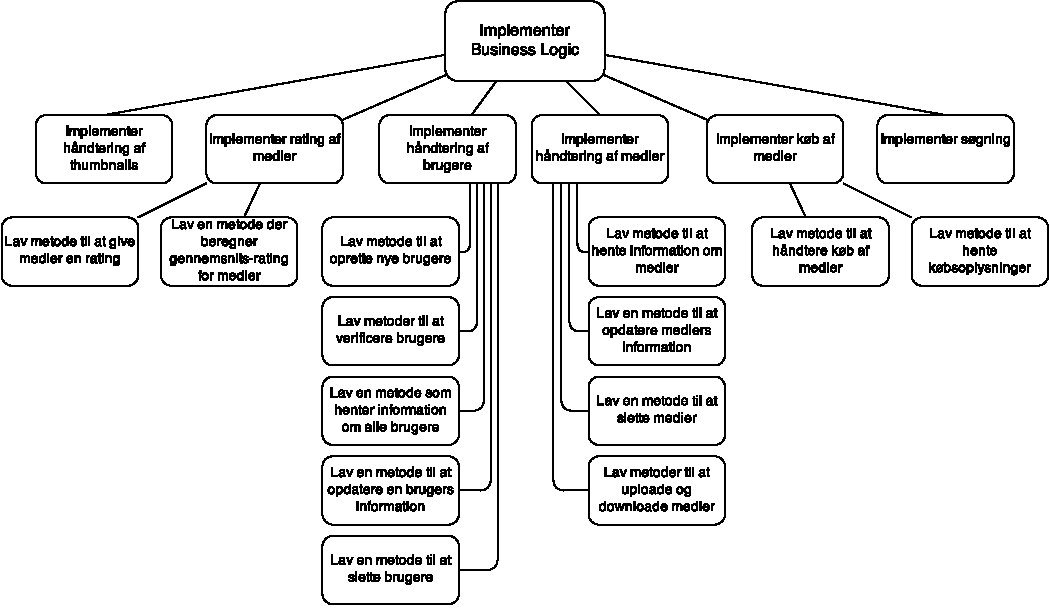
\includegraphics[scale=1.1]{BreakdownOfImplenterBusinessLogic.pdf}
\caption{Eksempel p� en aktivitet der er blevet brudt helt ned}
\label{fig:Full Breakdown Diagram}
\end{figure}

\noindent
Da Activity Breakdown Diagrammet, der blev lavet i target-projektet, ikke er brudt helt ned i atomiske aktiviteter, blev det ikke brugt til en dataljeret estimering af projektet, men mere til at planl�gge hvilke aktiviteter der skulle udf�res f�rst. Der blev ogs� lavet et Gantt-chart, som ud over at beskrive den r�kkef�lge aktiviteterne skulle udf�res i ogs� indeholdte en l�s tidsplan for projektet baseret p� Activity Breakdown Diagrammet.

\newgeometry{left=5cm,bottom=1.4cm}
\begin{landscape}


\begin{figure}[H]
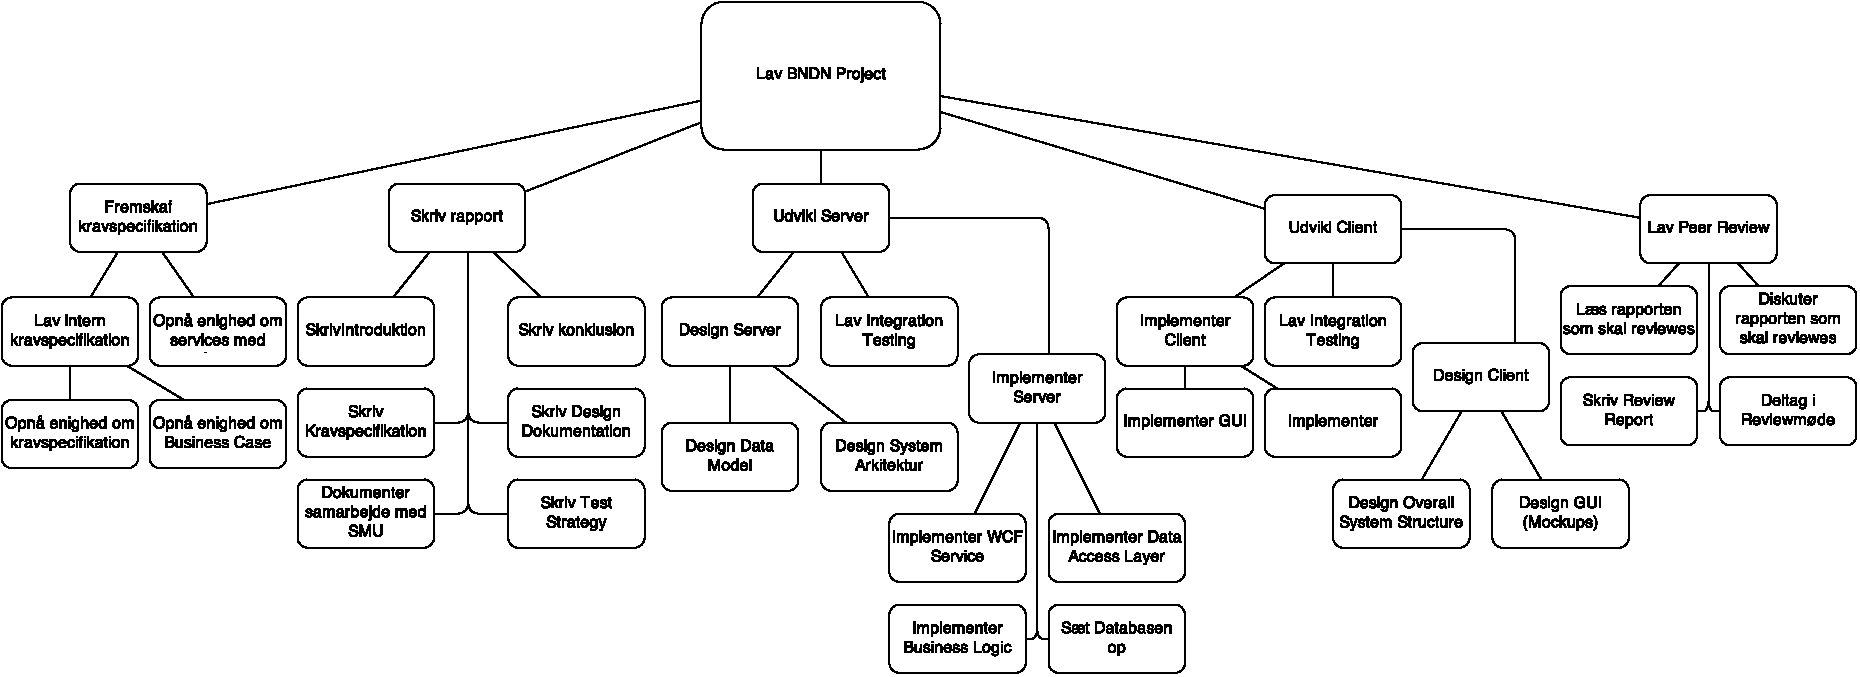
\includegraphics[ scale=0.86]{ActivityBreakdownDiagram.pdf}
\caption{Activity Breakdown Diagram fra target-projektet}
\label{fig:Activity Breakdown Diagram}
\end{figure}

\end{landscape}

\end{document}